\section{Exponential Functions, Logarithms and e}

\begin{frame}{Bacterial Growth on the Human Body}
  \begin{itemize}
    \item Our skin (and other areas like the mouth, nose, and intestines) hosts hundreds of thousands of microscopic organisms.
    \item In fact, bacterial cells in our body outnumber our own cells.
    \item While some bacteria can cause illness, many are essential for our health.
    \item Bacteria reproduce through binary fission—each cell splits into two.
    \item Under ideal conditions, a single bacterium doubling every hour can lead to over 1,000 cells in 10 hours and more than 16 million in 24 hours.
  \end{itemize}
\end{frame}

\begin{frame}{Bacterial Growth Over Time}
  \begin{table}[ht]
    \centering
    \begin{tabular}{c|ccccccccccc}
      \textbf{Hour} & 0 & 1 & 2 & 3 & 4 & 5 & 6 & 7 & 8 & 9 & 10 \\ \hline
      \textbf{Bacteria} & 1 & 2 & 4 & 8 & 16 & 32 & 64 & 128 & 256 & 512 & 1024 \\
    \end{tabular}
    \caption{Bacterial cell count doubling every hour.}
  \end{table}
\end{frame}

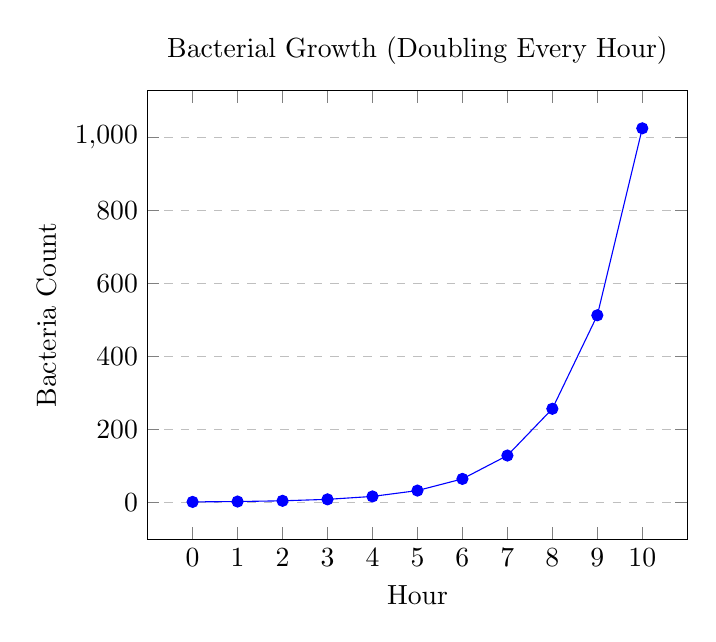
\begin{tikzpicture}
  \begin{axis}[
      xlabel={Hour},
      ylabel={Bacteria Count},
      title={Bacterial Growth (Doubling Every Hour)},
      xtick={0,1,2,3,4,5,6,7,8,9,10},
      ymajorgrids=true,
      grid style=dashed,
      % Uncomment the following line for a logarithmic scale on the y-axis:
      % ymode=log,
    ]
    \addplot[
      color=blue,
      mark=*,
      ]
      coordinates {
        (0,1) (1,2) (2,4) (3,8) (4,16) (5,32) (6,64) (7,128) (8,256) (9,512) (10,1024)
      };
  \end{axis}
\end{tikzpicture}

\begin{frame}{Population Growth in India}
  \begin{itemize}
    \item India is the second most populous country, with about 1.39 billion people in 2021.
    \item Its population grows at an annual rate of roughly 1.2\%.
    \item If this trend continues, India's population is projected to exceed China’s by 2027.
    \item While rapid population increases are often described as "exponential," in mathematics the term has a very precise meaning.
  \end{itemize}
\end{frame}

\begin{frame}{Defining Exponential Growth}
  \begin{block}{Key Concepts}
    \begin{itemize}
      \item \textbf{Percentage Change:} 
      \begin{itemize}
        \item refers to a change based on a percent of the original amount
      \end{itemize}
      \item \textbf{Exponential Growth:} 
        \begin{itemize}
          \item refers to an increase based on a constant multiplicative rate of change over equal increments of time, that is, a percent increase of the original amount over time.
          \item For example, if a quantity doubles each period, that is a 100\% increase per period.
        \end{itemize}
      \item \textbf{Linear Growth:} 
        \begin{itemize}
          \item The original value increases by a fixed \textbf{amount} (additive rate) over equal time intervals.
        \end{itemize}
        \item \textbf{Exponent Decay:}
        \begin{itemize}
          \item refers to a decrease based on a constant multiplicative rate of change over equal increments of time, that is, a percent decrease of the original amount over time.
        \end{itemize}
    \end{itemize}
  \end{block}
\end{frame}

\begin{frame}{Exponential Function and Its Behavior}
  \begin{block}{Definition}
    Suppose \(b>0\) with \(b\neq 1\). Then the \emph{exponential function} with base \(b\) is defined by
    \[
      f(x)=b^x.
    \]
    For example, if \(b=2\), then \(f(x)=2^x\). (Note that \(2^x\) is different from \(x^2\).)
  \end{block}
  \vspace{0.5em}
  \begin{block}{Behavior (for \(b>1\))}
    \begin{itemize}
      \item \textbf{Domain:} All real numbers, \(\mathbb{R}\).
      \item \textbf{Range:} All positive numbers, \((0,\infty)\).
      \item \(f(x)=b^x\) is an \emph{increasing} function.
      \item \(b^x\) becomes very large as \(x\) increases.
      \item \(b^x\) approaches \(0\) as \(x\) becomes very negative.
    \end{itemize}
  \end{block}
\end{frame}

\begin{frame}{Comparing Exponential and Linear Growth}
  \begin{table}[ht]
    \centering
    \begin{tabular}{c|c|c}
      \(x\) & \(f(x)=2^x\) & \(g(x)=2x\) \\ \hline
      0 & 1 & 0 \\
      1 & 2 & 2 \\
      2 & 4 & 4 \\
      3 & 8 & 6 \\
      4 & 16 & 8 \\
      5 & 32 & 10 \\
      6 & 64 & 12 \\
    \end{tabular}
    \caption{Exponential vs. Linear Growth.}
  \end{table}
\end{frame}


\begin{frame}{Example: The Function \(f(x)=2^x\)}
  \begin{block}{Exponential Growth Illustrated (Table 2)}
    \begin{table}[ht]
      \centering
      \begin{tabular}{|c|c|c|c|c|c|c|c|}
        \hline
        \(x\)      & -3 & -2 & -1 & 0 & 1 & 2 & 3 \\ \hline
        \(2^x\) & \(2^{-3}=\frac{1}{8}\) & \(2^{-2}=\frac{1}{4}\) & \(2^{-1}=\frac{1}{2}\) & \(2^0=1\) & \(2^1=2\) & \(2^2=4\) & \(2^3=8\) \\ \hline
      \end{tabular}
      \caption{Exponential values of \(2^x\) for \(x=-3,\dots,3\).}
    \end{table}
  \end{block}
  \vspace{1em}
  \textbf{Observation:} As \(x\) increases by 1, the output of \(2^x\) doubles, clearly illustrating exponential growth.
\end{frame}




\begin{frame}{Algebraic Properties of Exponents}
  \begin{block}{Properties}
    Let \(a, b > 0\) and \(x, y \in \mathbb{R}\). Then:
    \begin{itemize}
      \item \(b^x \cdot b^y = b^{x+y}\)
      \item \((b^x)^y = b^{xy}\)
      \item \(a^x \cdot b^x = (ab)^x\)
      \item \(b^0 = 1\)
      \item \(b^{-x} = \dfrac{1}{b^x}\)
      \item \(\dfrac{b^x}{b^y} = b^{x-y}\)
      \item \(\dfrac{a^x}{b^x} = \Bigl(\dfrac{a}{b}\Bigr)^x\)
    \end{itemize}
  \end{block}
\end{frame}

\begin{frame}
  \frametitle{Exponent Graph}
  \begin{columns}
    \begin{column}{0.5\textwidth}
      \begin{figure}
        \centering 
        \includegraphics[scale=0.3]{exp-vs-poly1.png}
       \end{figure}      
    \end{column}
 

    \begin{column}{0.5\textwidth}
      \begin{figure}
        \centering 
        \includegraphics[scale=0.2]{exp-vs-poly2.png}
       \end{figure}      
    \end{column}
  \end{columns}
\end{frame}


  \begin{frame}{Logarithm}
    \begin{block}{Definition}
      Suppose \(b\) and \(y\) are positive numbers with \(b\neq 1\). 
      \begin{itemize}
        \item The logarithm base \(b\) of \(y\), denoted \(\log_b y\), is defined as the unique number \(x\) such that
        \[
          b^x = y.
        \]
        \item  Short Version
        \[
          \log_b y = x \quad \text{means} \quad b^x = y.
        \]
      \end{itemize}
    \end{block}
  \end{frame}

  \begin{frame}{Logarithm of 1 and the Base}
    \begin{block}{Key Properties}
      Let \(b>0\) with \(b\neq 1\). Then:
      \begin{itemize}
        \item \(\log_b 1 = 0\) because \(b^0 = 1\),
        \item \(\log_b b = 1\) because \(b^1 = b\).
      \end{itemize}
    \end{block}
  \end{frame}

  \begin{frame}{Logarithm as an Inverse Function}
    \begin{block}{Definition}
      Suppose \(b\) is a positive number with \(b \neq 1\) and the exponential function \(f\) is defined by
      \[
        f(x) = b^x.
      \]
      Then the inverse function \(f^{-1}\) is given by
      \[
        f^{-1}(y) = \log_b y.
      \]
    \end{block}
  \end{frame}
  
  \begin{frame}{Inverse Properties of Logarithms - Summary}
    \begin{itemize}
      \item \textbf{Inverse Relationship:}
        \begin{itemize}
          \item \(\log_b x\) is the inverse of \(b^x\).
          \item Flipping the graph of \(b^x\) across the line \(y=x\) yields the graph of \(\log_b x\).
        \end{itemize}
      \item \textbf{Monotonicity:}
        \begin{itemize}
          \item For \(b>1\), \(b^x\) is increasing, so \(\log_b x\) is also increasing.
        \end{itemize}
      \item \textbf{Key Equations:}
        \begin{itemize}
          \item \(b^{\log_b y} = y\)
          \item \(\log_b (b^x) = x\)
        \end{itemize}
      \item \textbf{Function-Inverse Properties:}
        \begin{itemize}
          \item These can be written as \((f \circ f^{-1})(y) = y\) and \((f^{-1} \circ f)(x) = x\).
        \end{itemize}
      \item \textbf{Understanding:}
        \begin{itemize}
          \item These properties are fundamental to the relationship between exponential and logarithmic functions.
        \end{itemize}
    \end{itemize}
  \end{frame}

  \begin{frame}{Logarithm of a Power}
    \begin{block}{Property}
      If \(b\) and \(y\) are positive numbers, with \(b \neq 1\), and \(t\) is a real number, then
      \[
        \log_b\left(y^t\right) = t \log_b y.
      \]
    \end{block}
  \end{frame}